\documentclass[final]{beamer}

% ====================
% Packages
% ====================

\usepackage[T1]{fontenc}
\usepackage{lmodern}
\usepackage[size=custom,width=120,height=72,scale=1.0]{beamerposter}
\usetheme{gemini}
\usecolortheme{gemini}
\usepackage{graphicx}
\usepackage{booktabs}
\usepackage{tikz}
\usepackage{xcolor}
\usepackage{pgfplots}
\pgfplotsset{compat=1.7}

% ====================
% Lengths
% ====================

% If you have N columns, choose \sepwidth and \colwidth such that
% (N+1)*\sepwidth + N*\colwidth = \paperwidth
\newlength{\sepwidth}
\newlength{\colwidth}
\setlength{\sepwidth}{0.025\paperwidth}
\setlength{\colwidth}{0.3\paperwidth}

\newcommand{\separatorcolumn}{\begin{column}{\sepwidth}\end{column}}

% ====================
% Title
% ====================

\title{DESCRIBING THE WOBBLING MOTION IN \texorpdfstring{$^{163}$}{163}Lu THROUGH A SEMI-CLASSICAL APPROACH}

\author{Robert Poenaru \inst{1,2} | \texttt{robert.poenaru@protonmail.ch}}

%\institute[shortinst]{\inst{1} Doctoral School of Physics, University of Bucharest, Bucharest, Romania \samelineand \inst{2} Department of Theoretical Physics, Horia-Hulubei National Institute of Nuclear Physics and Engineering, Bucharest-Magurele, Romania}

\institute[shortinst]{\inst{1} Doctoral School of Physics, University of Bucharest, Bucharest, Romania \\ \inst{2} Department of Theoretical Physics, Horia-Hulubei National Institute of Nuclear Physics and Engineering, Bucharest-Magurele, Romania}

% ====================
% Body
% ====================

\begin{document}

\addtobeamertemplate{headline}{} 
{\begin{tikzpicture}[remember picture, overlay]
     \node [anchor=north east, inner sep=0.9cm]  at (current page.north east)
     {
\includegraphics[height=10cm]{./images/logos/logo.png}};
     \node [anchor=north west, inner sep=0.9cm]  at (current page.north west)
     {
\includegraphics[height=9cm]{./images/logos/uniLogo.png}};
  \end{tikzpicture}}
  
\begin{frame}[t]
\begin{columns}[t]
\separatorcolumn
\begin{column}{\colwidth}
  \begin{block}{Introduction}

\heading{Motivation}

\heading{Research goals}

  \end{block}
\begin{block}{Wobbling Motion in Nuclei}
  Wobbling motion in nuclei employs a \emph{precession} of the total angular momentum combined with an \emph{oscillation} of its projection onto the rotational axis. Different \emph{core-particle} couplings lead to different wobbling regimes (See Fig. \ref{wobbling-regimes}).
  \begin{figure}
      \centering
     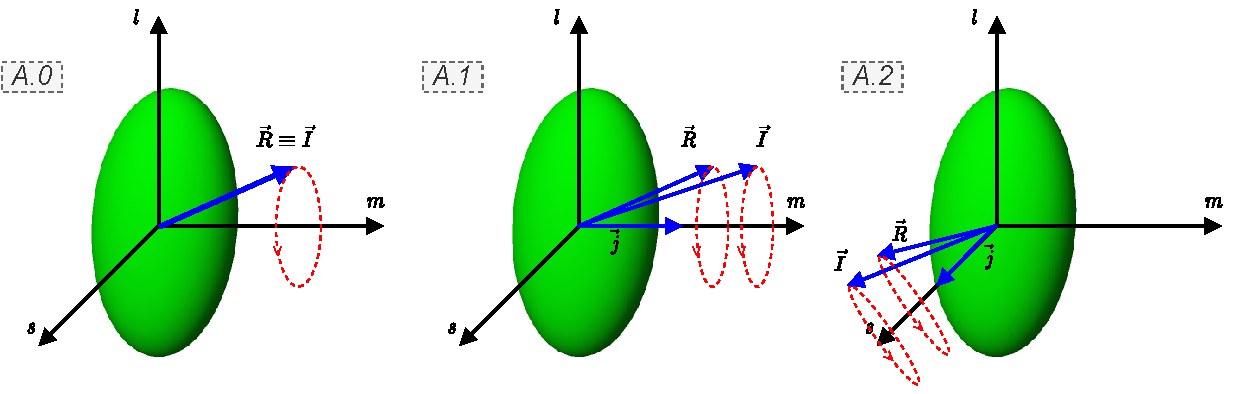
\includegraphics[scale=1.7]{images/wobbling_Regimes_COUPLING_SCHEME.pdf}
      \caption{An illustration with the wobbling regimes which can occur in a nucleus. From left to right: \emph{simple/ideal wobbler}, \emph{longitudinal wobbler}, \emph{transverse wobbler}.}
      \label{wobbling-regimes}
  \end{figure}
  \begin{figure}
      \centering
     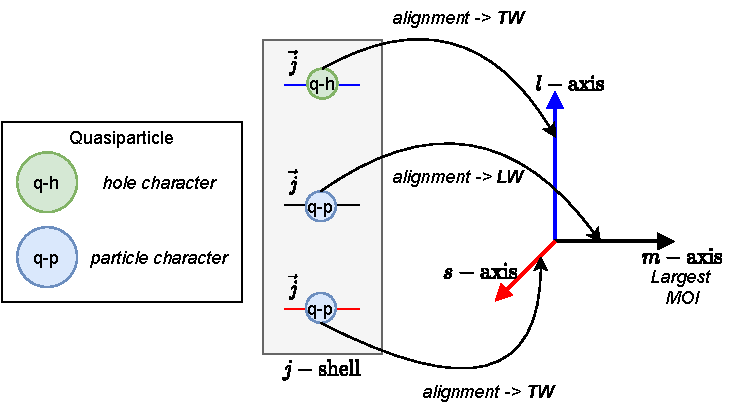
\includegraphics[scale=2.2]{images/wobbling_Regimes_updated.pdf}
      \caption{An illustration with the wobbling regimes which can occur in a nucleus. From left to right: \emph{simple/ideal wobbler}, \emph{longitudinal wobbler}, \emph{transverse wobbler}.}
      \label{tw-lw-wobbling}
  \end{figure}

\end{block}
\end{column}
\separatorcolumn
\begin{column}{\colwidth}
  \begin{block}{Odd-A Formalism}
The system is described by the total PRM Hamiltonian:
\begin{align}
    \hat{H}=\hat{H}_\text{core}+\hat{H}_\text{sp}\ ,
\end{align}
where $\hat{H}_\text{core}$ describes the dynamics of the triaxial core, and $\hat{H}_\text{s.p.}$ is the single-particle potential that corresponds to the odd nucleon. Depending on the angular momentum $\vec{j}$ of the nucleon, and the strength parameter $V$, its expression corresponds to a Nilsson potential as such:
\begin{align}
\hat{H}_\text{sp}&\equiv V_\text{sp}=\frac{\mathbf{V}}{j(j+1)}\left[\cos\gamma Y_{20}+\frac{\sin\gamma}{\sqrt{2}}\left(Y_{2-2}+Y_{22}\right)\right]\ .
\end{align}
  \end{block}
    \begin{block}{Results}
  \begin{figure}
\centering
\begin{minipage}{.5\textwidth}
  \centering
  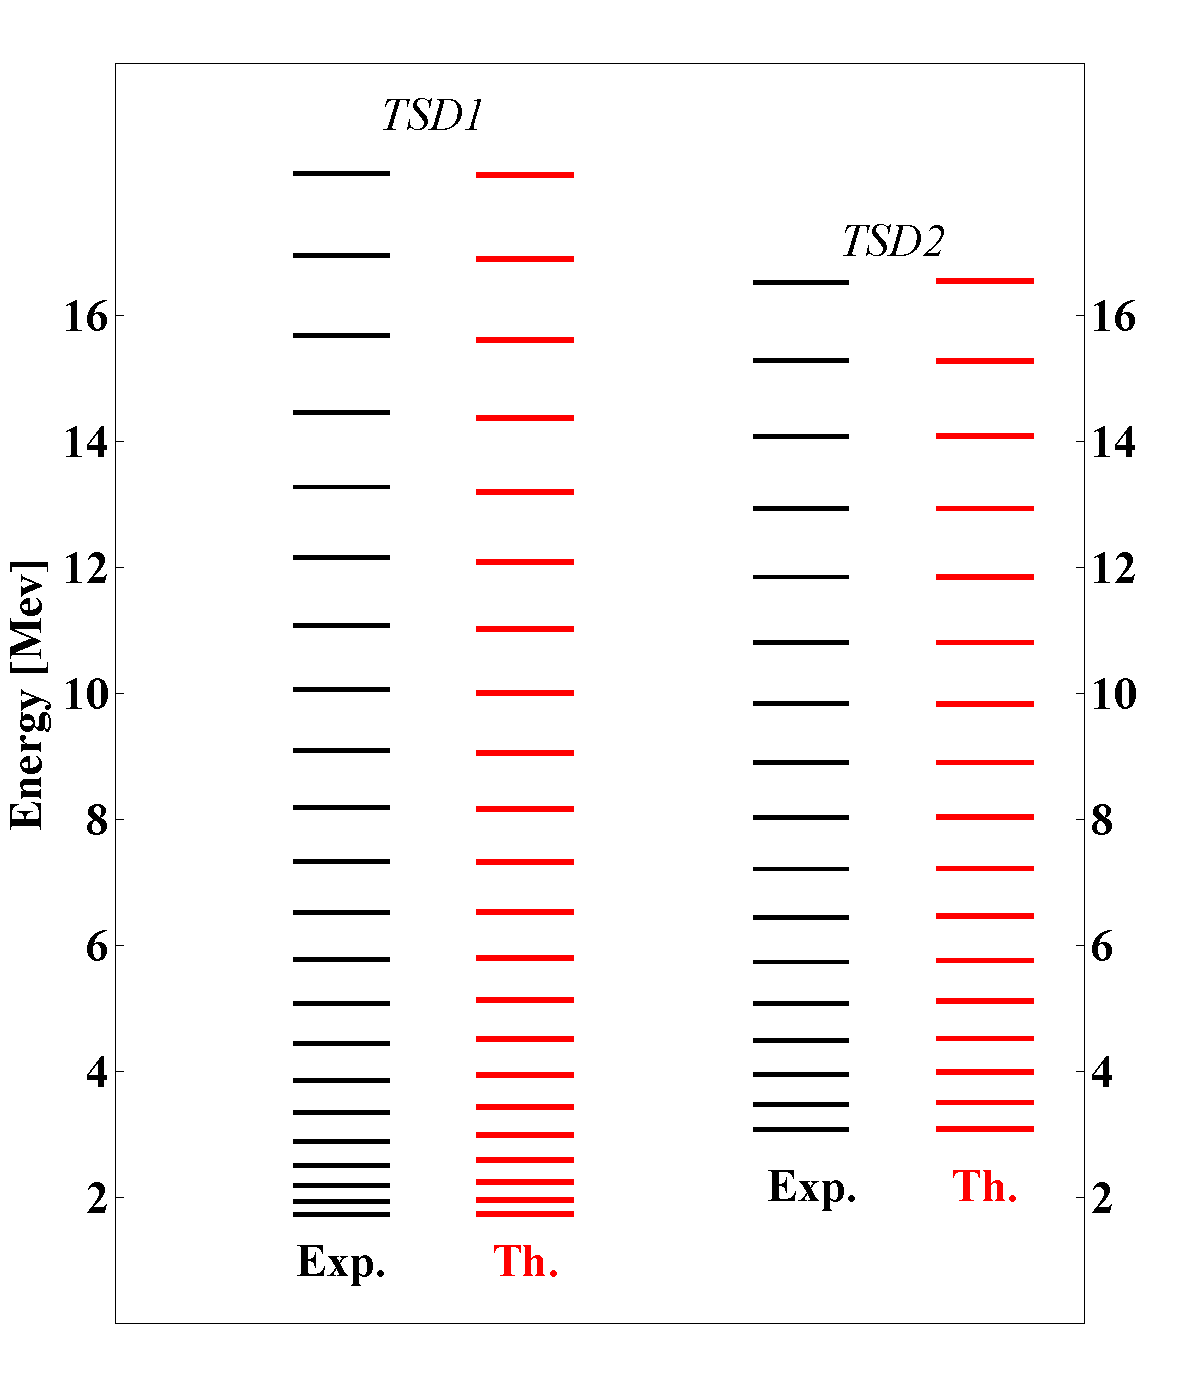
\includegraphics[scale=0.85]{images/TSD-12.pdf}
\end{minipage}%
\begin{minipage}{.5\textwidth}
  \centering
 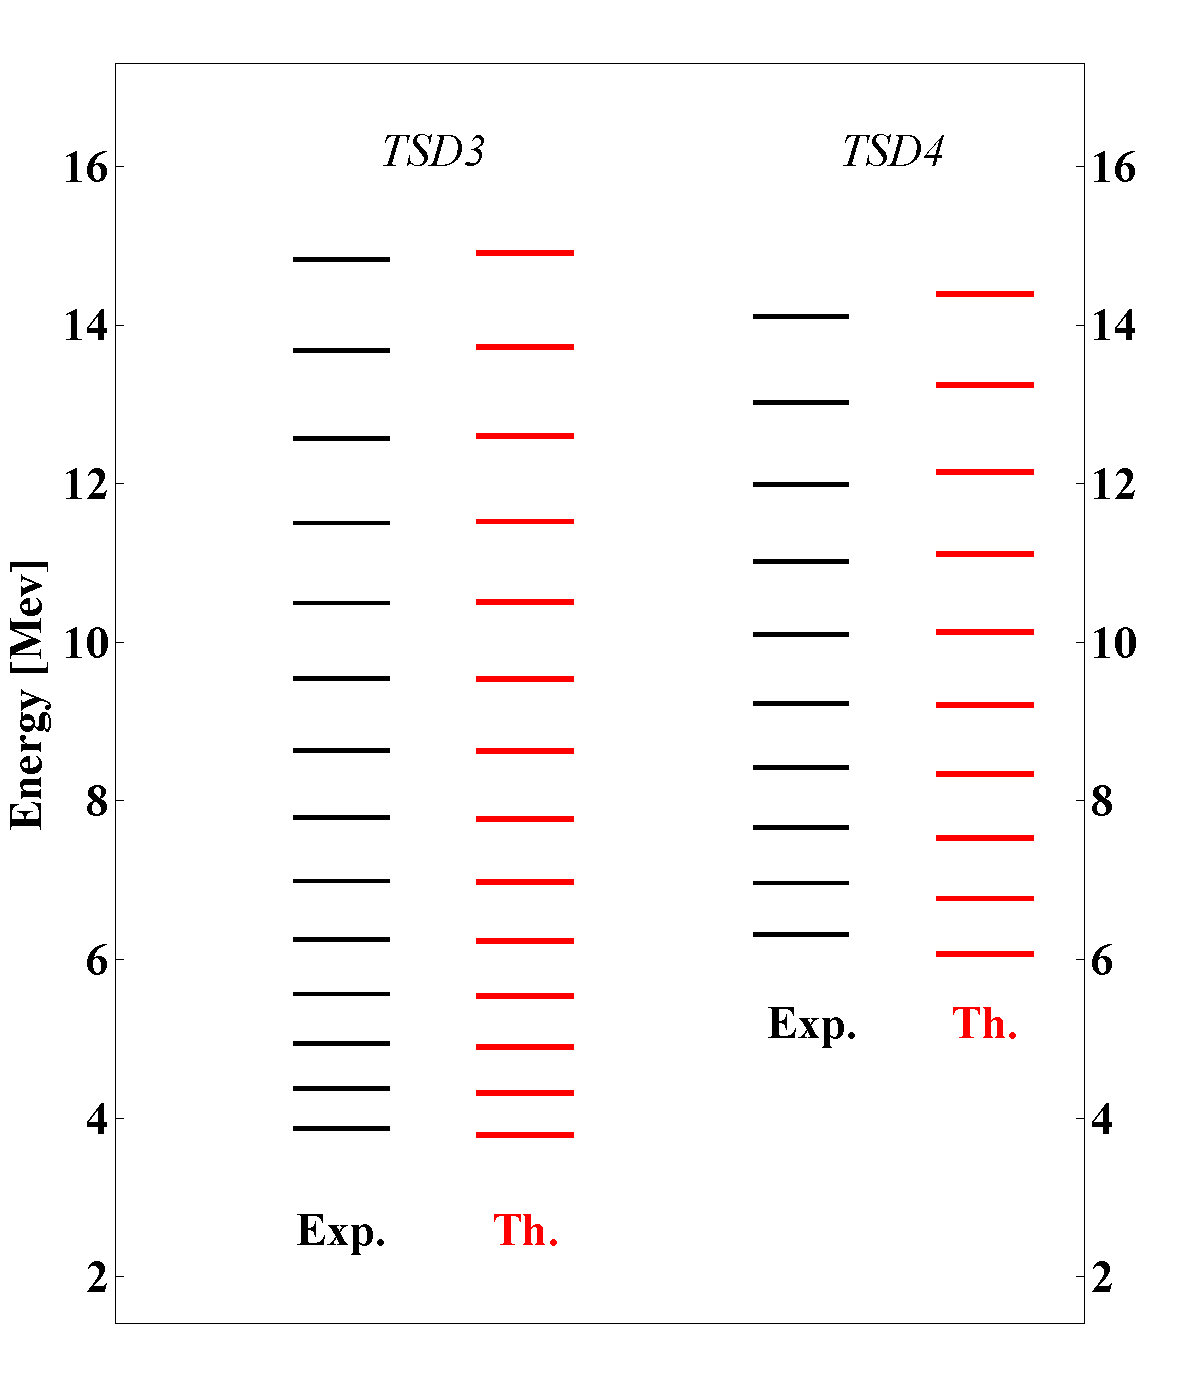
\includegraphics[scale=0.85]{images/TSD-34.pdf}
\end{minipage}
\caption{\textbf{Left:} ideal wobbler (case $A.0$ depicted above). \textbf{Right:} real wobbling spectrum of $^{163}$Lu (case $A.2$ depicted above).}
    \label{energy-function-min-point-evolution}
\end{figure}
  \end{block}
\end{column}
\separatorcolumn
\begin{column}{\colwidth}
    \begin{block}{Conclusions}

  \end{block}
%   \begin{block}{References}

%     \nocite{*}
%     \tiny{\bibliographystyle{plain}\bibliography{poster}}

%   \end{block}
\end{column}

\separatorcolumn

\end{columns}

\end{frame}

\end{document}